\chapter{Arbeitspakete}
Die einzelnen Arbeitspakete werden Mithilfe vom Projektverwaltungstools Redmine organisiert. Für die Betreuer wurde ein eigener Zugang zum Redmine-Projekt eingerichtet.

\section{Gastzugang Redmine}
http://152.96.192.44/redmine \\
Zugang: guest / zurich2Rapperswil \\

\section{Arbeitspakete}
	\begin{figure}[H]
		%\centering
		% trim=links unten rechts oben
		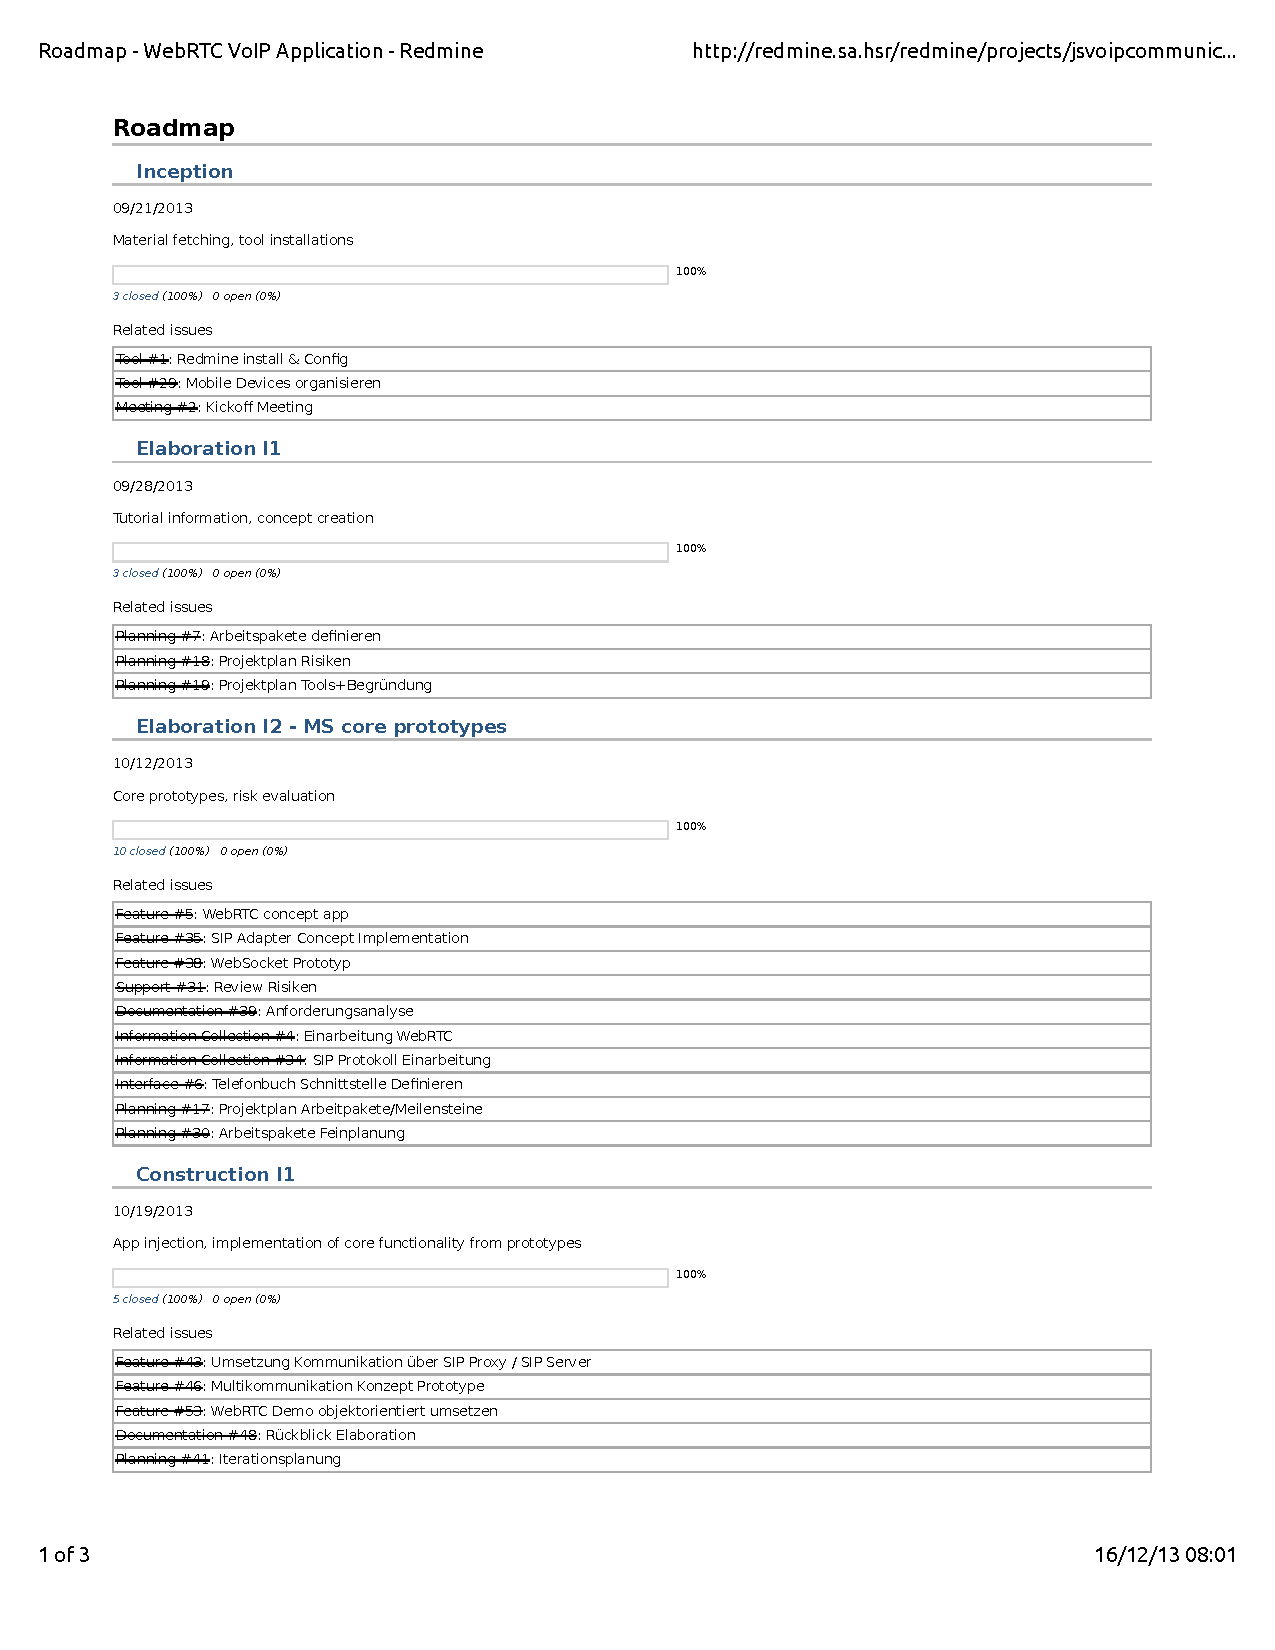
\includegraphics[trim=1.75cm 2cm 2cm 2.5cm, clip=true,page=1,width=0.88\textwidth]{media/roadmap.pdf}
		%\caption[Roadmap]{Arbeitspakete und Milestones}
		%\label{roadmap}
	\end{figure}

	\begin{figure}[H]
		%\centering
		% trim=links unten rechts oben
		\includegraphics[trim=1.75cm 2cm 2cm 2.5cm, clip=true,page=2,width=0.88\textwidth]{media/roadmap.pdf}
		%\caption[Roadmap]{Arbeitspakete und Milestones}
		%\label{roadmap}
	\end{figure}

	\begin{landscape}
	\subsection{Gantt}
		\begin{figure}[H]
			\centering
			% trim=links unten rechts oben
			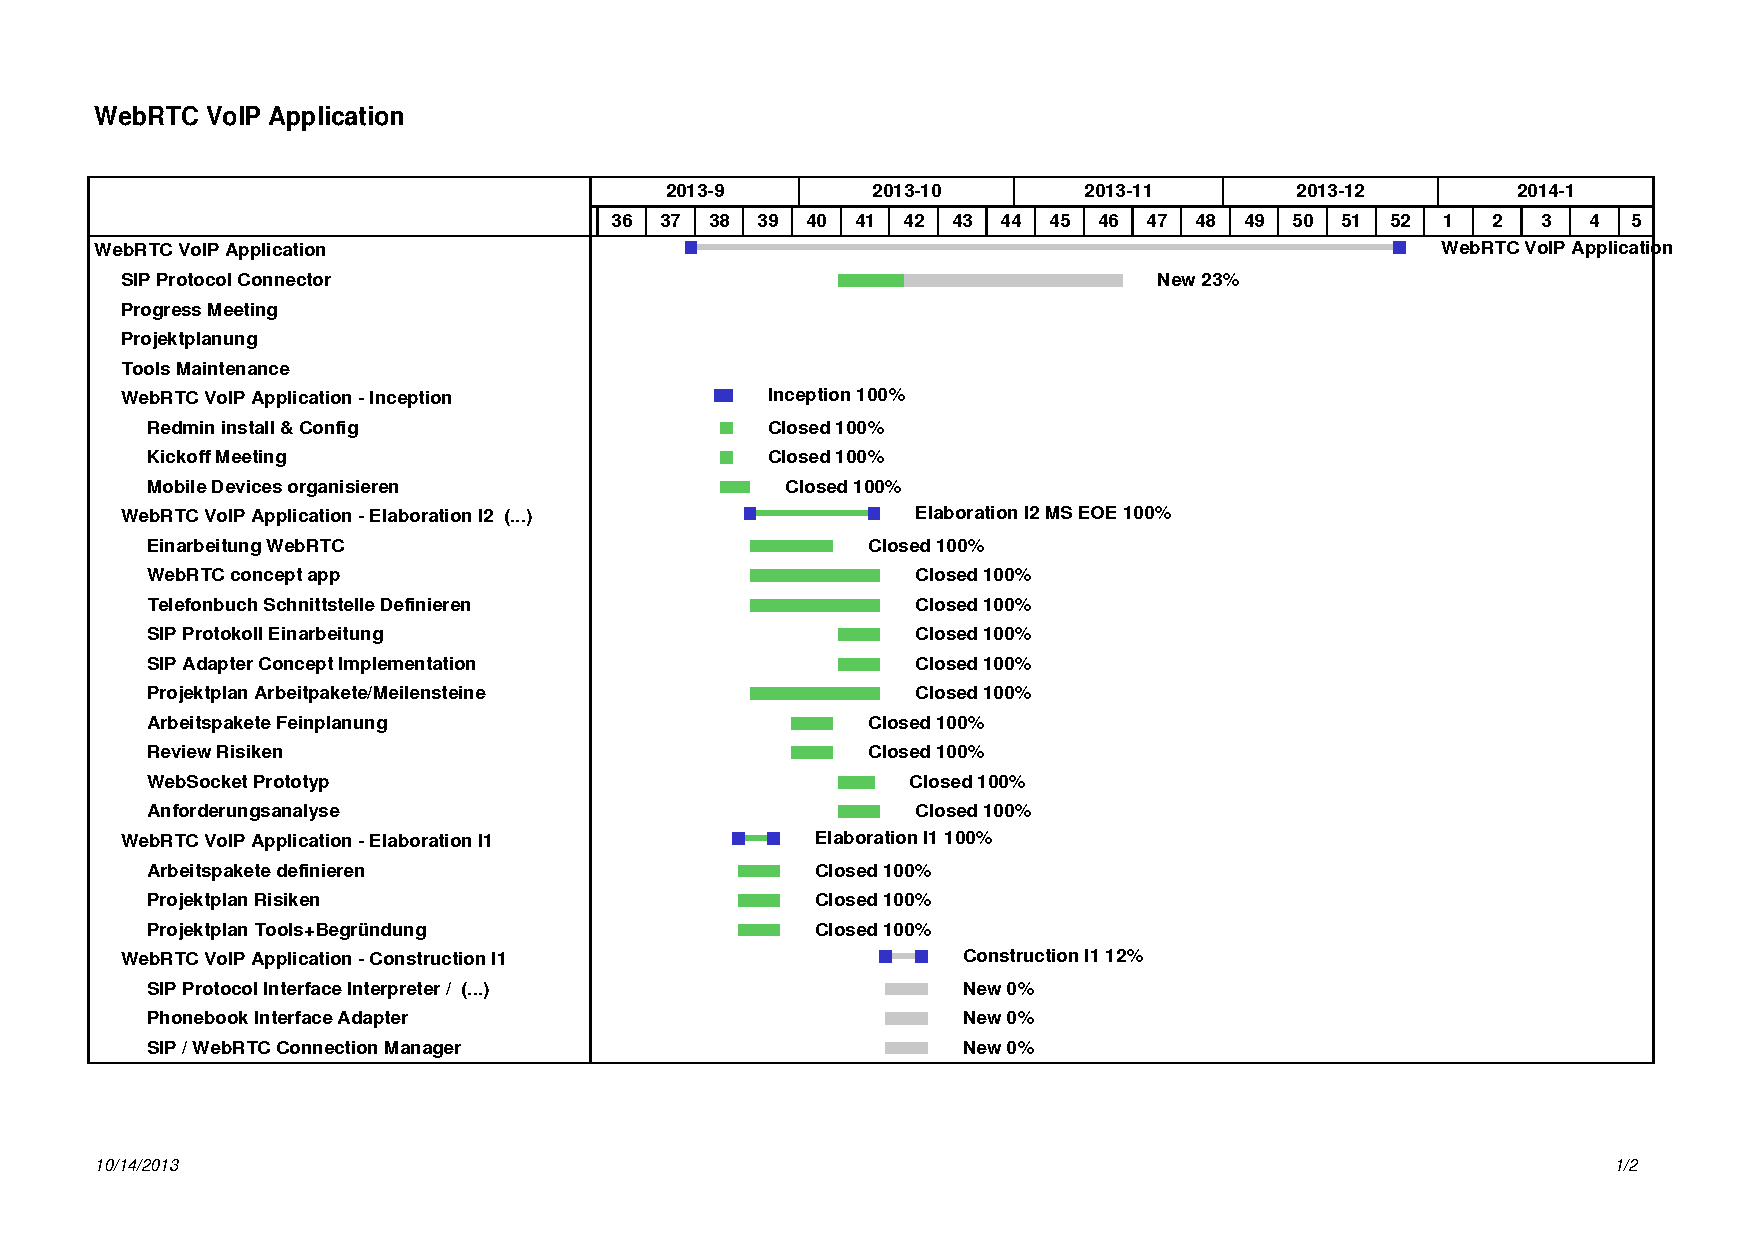
\includegraphics[trim=1.5cm 2.5cm 1cm 3cm, clip=true,page=1,width=1.4\textwidth]{media/jsvoipcommunication-gantt.pdf}
			\caption[Gantt]{Gantt}
			\label{gantt}
		\end{figure}
		\begin{figure}[H]
			\centering
			% trim=links unten rechts oben
			\includegraphics[trim=1.5cm 2.5cm 1cm 1cm, clip=true,page=2,width=1.4\textwidth]{media/jsvoipcommunication-gantt.pdf}
			\caption[Gantt]{Gantt}
			\label{gantt}
		\end{figure}
	\end{landscape}
